% Beispiel für Klasse tudposter.cls (Version 0.5).
%%
%% Autor: Martin Zabel (martin.zabel@tu-dresden.de)
%%        Tobias schlemmer (tobias.schlemmer@mailbox.tu-dresden.de)
%%
%% Klassenoptionen siehe tudposter.cls.
%%
%%
%% Wir bevorzugen PDFLaTeX. Für den Fall, dass die CD-Schriften nicht
%% in der Standardkonfiguration erwähnt sind laden wir die .map-Datei
%% Wichtig: das muss vor dem ersten Font-Befehl (also vor der
%% Dokumentklasse geschehen.
%
% Diese Zeilen sind jetzt auskommentiert, da dies das Paket „tudfonts“
% jetzt übernimmt
%
%\pdfmapfile{+univers.map}
%\pdfmapfile{+dinbold.map}
%%
\documentclass[a0paper,noDIN,MathematikA0]{tudmathposter}
\listfiles
% Bei Bedarf: dinBold für Section. Dann aber auch Überschrift nur in
% Großbuchstaben.
%\addtokomafont{section}{\dinBold}

% In diesem Poster benötigte Pakete.
% Jedem wie es beliebt.
\usepackage[T1]{fontenc}
\usepackage[utf8]{inputenc} % latin1 (Linux) oder ansinew (Win) wenn
                            % nicht UTF 8
\usepackage[ngerman]{babel}
\usepackage{multicol}
\usepackage{listings}
\usepackage{tikz}
\usepackage{url}
\usepackage[pdfborder={0 0 0}]{hyperref}
%\usepackage{tabularx}
\usetikzlibrary{calc}
\usetikzlibrary{shapes.multipart}
\usetikzlibrary{positioning}

% Beispiel für die Verwendung des listings-Paketes (Mutabor-Sprache)
\lstdefinelanguage{Mutabor}{%
%otherkeywords={:,=,:=,+,-,*,\(,\),[,],.,\,,;},
%morekeywords=[1]{},%
%Befehle
morekeywords=[1]{INTERVALL,TON,TONSYSTEM,UMSTIMMUNG,HARMONIE,LOGIK,%
INTERVAL,TONE,TONESYSTEM,RETUNING,PATTERN,LOGIC,SHIFTED},%
%Funktionen
morekeywords=[2]{MIDIKANAL,WURZEL,TASTE,MIDIIN,MIDIOUT,ANSONSTEN,%
FORM,ROOT,MIDICHANNEL,KEY,ELSE},
%morekeywords=[3]{=,-},
%Datentypen
%morekeywords=[4]{},%
   sensitive=false,%
   %alsoletter={=,-},
%   alsoletter={+,-,*,/,.,:,=,<,>}, %(,),[,],.,\,,:,;,^,@,
%   morecomment=[s]{(*}{*)},%
%   morecomment=[s]{\{}{\}},%
%   morecomment=[l]{//},%
   morecomment=[s]{"}{"},%
%   moredelim=*[s]{\[}{\]},%
%   moredelim=*[s]{(}{)}
%   moredelim=*[s]{\{}{\}}
%   morestring=[d]'%
  }%[keywords,comments,strings]%
% lst-Sprachen laden.
\lstloadlanguages{Mutabor}
% Einstellungen für listings: Fonts und Farben
\lstset{%
  tabsize=8,
  language=Mutabor,
  defaultdialect=Mutabor,
  basicstyle=\ttfamily\scriptsize\normalcolor,
  identifierstyle=\color{HKS92K100},
  keywordstyle=[1]{\color{HKS41K100}\bfseries},
  keywordstyle=[2]{\color{HKS41K100}},
  keywordstyle=[4]{\normalcolor},
  keywordstyle=[3]{\color{HKS92K100}},
  stringstyle=\color{HKS92K50},
  commentstyle=\color{HKS92K70}\textit,
  inputencoding=utf8,
  extendedchars=false,
  showtabs=false,
  showspaces=false,%
  texcl=true,%
  escapechar=",
  escapebegin={\color[rgb]{0.5,0.5,0.5}\expandafter\textit\bgroup%
    \obeylines\obeyspaces
    \dq},
  escapeend={\dq\egroup}
}

\newlength{\zielbreite}%
\newlength{\zielhoehe}%
\newlength{\printmml}%

% Beschriftung im Seitenkopf und Seitenfuß
\institut{Institut für Algebra}
\professur{Professur für \TeX nische Algebra}
\author{T. Schlemmer, M. Behrisch und D. Borchmann\\\strut}% Zum Beispiel für Kontaktdaten.
\telefon{0351 463-35078\\\strut}
\fax{0351 463-\dots}
\email{Tobias.Schlemmer@mailbox.tu-dresden.de}
\homepage{\url{http://www.math.tu-dresden.de/~schlemme/tudmathposter/}}
% Folgende Zeile ist nicht CD-konform
\institutslogofile{mathelogo}

\title{Die Dokumentklasse „tudmathposter“}
\subtitle{Eine \LaTeX klasse für die Evaluationsposter}
\grautabelle
\addto\captionsngerman{%
  \def\figurename{Abb.}%
  \def\tablename{Tab.}%
}%
\begin{document}
%\color{HKS41K100}%
%%%%%%%%%%%%%%%%%%%%%%%%%%%%%%%%%%%%%%%%%%%%%%%%%%%%%%%%%%%%%%%%%%%%%%%%%%%%
%%% Poster-Titel
%%%%%%%%%%%%%%%%%%%%%%%%%%%%%%%%%%%%%%%%%%%%%%%%%%%%%%%%%%%%%%%%%%%%%%%%%%%%
\maketitle
%%%%%%%%%%%%%%%%%%%%%%%%%%%%%%%%%%%%%%%%%%%%%%%%%%%%%%%%%%%%%%%%%%%%%%%%%%%%
%%% Poster-Inhalt

\section{Hinweise zur Klasse}
\begin{multicols}{2}%
Die Dokumentklasse „tudmathposter“ wurde für die Vorbereitung von
Postern anlässlich der Evaluation 2010 des Fachbereiches Mathematik
der TU Dresden aufgesetzt. Sie basiert auf der Beispielklasse des
CD-Büros der TUD von Martin Zabel.

\subsection{Aufruf}

{\small\textbackslash
documentclass[noDIN,a0paper,Mathematik]\{tudmathposter\}}

Die Klassenoptionen sind mit anzugeben. Andernfalls fällt die Klasse
in einigen Einstellungen auf das Standard-CD der TUD zurück.
\subsection{Neue Kommandos}
\begin{description}
\item[\textbackslash tudfont\{font\}] wählt eine der Univers-Varianten
  der TUD (siehe Tab. \ref{tab:schriften}aus. Hinweis: Der Schriftschnitt „Univers 45 Light Bold“
  wird nicht mit ausgeliefert, sondern muss durch „Univers 60
  Bold“ ersetzt werden. Es sollte sich kein Problem ergeben.
\item[\textbackslash begin\{farbtabellen\}\dots\textbackslash
  end\{farbtabellen\}]
Innerhalb dieser Umgebung werden alle Tabellen farbig gesetzt ähnlich
Tabelle \ref{tab:schriften}. Die Tabellen müssen in eine angemessene
Tabellenumgebung (vorzugsweise tabularx) eingebettet werden. Es wurde bewusst darauf
verzichtet, eine eigene Umgebung zu definieren, um die Kreativität
nicht weiter zu beschränken.
\item[\textbackslash grautabelle und \textbackslash blautabelle]
  schaltet die Farben für die mehrfarbigen Tabellen um.
\item[\textbackslash color\{HKS$x$K$y$\}, \textbackslash textcolor\{HKS$x$K$y$\} usw.] Diese
  Makros wurden nicht neu definiert, wohl aber die Farben. Sie sind
  den Sonderfarben der HKS-Tabelle nachempfunden. Zur Auswahl stehen
  \[
  x\in\{41,92\}\text{ und } y\in \{10,20,30,40,50,60,70,80,100\}.
  \]
  Dabei
  steht der Wert $100$ für die unveränderte HKS-Farbe (die Farbe des
  CD) und die kleineren Werte sind abgeschwächte Werte für Tabellen,
  Zeichnungen etc. Die genauen Vierfarb-Werte können aus der
  Dokumentklasse entnommen werden. 

  Wenn die Sonderfarben zur Verfügung stehen, sollten wenigstens
  HKS41K100 und HKS92K100 in der PDF-Datei durch spezielle Sonderfarben
  ersetzt werden. Hierbei kann das \LaTeX-Paket spotcolor hilfreich
  sein (ungetestet, daher nicht angeboten).
\end{description}
\end{multicols}

\begin{table}[h]
  \begin{farbtabellen}
    \begin{tabularx}{\linewidth}{|X|X|X|}
      \rowcolor{HKS41K60}\textbf{\color{white}\rule{0pt}{1em}Spaltenüberschrift}&\textbf{\color{white}Spaltenüberschrift}&\textbf{\color{white}Spaltenüberschrift}\\\hline
Univers CE 75 Black&
Univers CE 75 Black Oblique&
Univers CE 60\\
Univers CE 60 Oblique&
Univers CE 45 Light&
Univers CE 45 Light Oblique\\
Univers CE 55&
Univers CE 55 Oblique&
Din Bold
    \end{tabularx}
  \end{farbtabellen}

  \caption{Mögliche Schriftarten für \textbackslash tudfont}
  \label{tab:schriften}
\end{table}

\begin{multicols}2
  \centersubsection{Weitere Makros}
  Eine ganze Reihe von weiteren Kommandos kann benutzt werden, um
  die Üblichen Angaben zu machen. Die Namen sollten selbsterklärend
  sein.

  Es sind \textbackslash title, \textbackslash subtitle,
  \textbackslash einrichtung, \textbackslash fachrichtung,
  \textbackslash institut, \textbackslash professur, \textbackslash
  telefon, \textbackslash \fax, \textbackslash homepage
  
  Ein Beispiel für die Benutzung sehen sie am Anfang dieser .tex-Datei.
  
  Einige dieser Makros sind sinnvoll vorbelegt.
  
  Das Makro
  \textbackslash fusszeile erlaubt es, den gesamten Seitenfuß
  umzudefinieren.
  \centersubsection {Schriften}
  Als Schriften stehen die Univers-Familie, sowie der fette
  Schriftschnitt von Din bereit. Entsprechend der Vorgabe des
  Prodekanates werden die Din-Schriften allerdings nicht
  verwendet. Dies wird über die Option „noDIN“ der Dokumentklasse
  mitgeteilt.

  Als Schriftgrößen stehen die normalen Größen von \textbackslash tiny
  bis \textbackslash Huge zur Verfügung. Dabei wurden zunächst die
  Größen aus der Vorgabe definiert und dann zusätzliche Größen
  interpoliert. Bei Verwendung der Standard-\LaTeX-Makros zur
  Textauszeichnug sollte die Schriftgröße automatisch richtig gesetzt
  werden.
  \enlargethispage{4\baselineskip}
\subsection{Geladene Pakete}
  Die Dokumentklasse basiert auf der Klasse „scrartcl“ aus dem
  KOMA-Skript-Paket. Dieses Paket hat sich als Standardklassen für
  europäischen Textsatz gegenüber den angelsächsischen Standardklassen
  durchgesetzt.

  Weiterhin werden die Pakete „calc“, „xcolor“, „graphicx“,
  „textcomp“, „tabularx“ und „lmodern“ nachgeladen. Es wird empfohlen,
  das Paket „multicols“ zu verwenden.

  \subsection{Team}
  Die Klasse wurde von Mike Behrisch, Daniel Borchmann und Tobias
  Schlemmer angepasst. Die Autoren stehen für Fragen bereit.
\end{multicols}
\pagebreak
\fax{}\label{Updanfang}%
\title{Updates III (Seiten \pageref{Updanfang} bis \pageref{Updende})}%
\subtitle{Änderungen an der Klasse für die neue Version}
\maketitle
\section{Version 2.0 (24.\,08.\,2012)}
Die Beamer-Stile wurden komplett überarbeitet. Ab jetzt wird für
Abwärtskompatibilität \emph{keinerlei} Haftung mehr übernommen. Ziel
ist es, brauchbare und schöne Vorlagen zu erstellen. Kapitelnummern
stehen jetzt vor der Kapitelüberschrift und nicht mehr vor der
Folienüberschrift. Seiten können nach Folien- oder Seitenzahl
nummeriert werden. Für Entwicklungszwecke gibt es die Möglichkeit,
innerhalb einer Folie die Bildnummern anzeigen zu lassen. Die
Dokumentation ist nicht mehr so sauber, wie bisher und Support ist
reine Kulanzssache.

\section{Version 1.10 (11.\,02.\,2011)}
Das Paket tudfonts kann nun dank Mike Behrisch auch in Dokumente
eingebunden werden, die kein
PDF-LaTeX verwenden. Bei Verwendung von dvips müssen die Optionen
„-u+univers.map“ und „-u+dinbold.map“ hinzugefügt werden, falls diese
nicht global geladen werden. Das Überschreiben im der Tabellen im
nutzerspezifischen texmf"=Baum kann zu Problemen führen, wenn global
Pakete aktualisiert bzw.\ installiert werden.
\section{Version 1.9 (18.\,10.~2010)}
Die Postleitzahl und der Ort Dresden wurden entfernt.

Aus \TeX nischen Gründen darf das Feld Homepage keine Zeilenumbrüche o.ä. enthalten. Eine entsprechende Fehlermeldung wurde hinzugefügt.
\section{Version 1.8 (15.\,10.~2010)}
\begin{multicols}2
\begin{itemize}
\item Absicherung des korrekten Fakultätsnamens
\item Schriftgrößen sind jetzt auch mit älteren Koma"=Skript"=Klassen kompatibel
\item Neues Fußzeilenfeld \textbf{\textbackslash email}
\item Offizielle Vorgaben für den Fußbereich wurden umgesetzt:
	\begin{itemize}
	\item 	Die \textbf{linke Spalte} enthält Hochschule, Einrichtung, Fachrichtung, Institut und 		Professur. 
		Institut und Professur sollten mit \textbf{\textbackslash institut} und 		\textbf{\textbackslash professur} gesetzt werden. Die restlichen, Einrichtung und 		Fachrichtung, werden automatisch gesetzt.
	\item 	Die \textbf{rechte Spalte} ist frei wählbar, und kann alternativ mit den vorgegebenen Variablen \textbf{\textbackslash author}, \textbf{\textbackslash telefon}, \textbf{\textbackslash email} und \textbf{\textbackslash homepage} oder mit einem frei gewählten Absatz (\textbf{\textbackslash footcolumn2}) gefüllt werden.
	
	\textbf{Hinweis:} Wenn sich die Homepage mit dem Institutslogo überschneidet, kann jedes beliebige Feld mit Zeilenumbrüchen vertikal erweitert werden. Dazu können die üblichen Makrokombinationen wie \textbackslash\textbackslash\ für den Zeilenumbruch und \textbackslash strut zum Erzeugen von Inhalt für eine leere Zeile genutzt werden.
	\end{itemize}
	\item Das Institutslogo erhält seine endgültige Position.
\end{itemize}
\end{multicols}
\section{Version 1.7 (21.\,09.~2010)}
\begin{multicols}2
Neues Dresden-Concept-Logo (voraussichtlich Endfassung)
\end{multicols}
\section{Version 1.6 (09.\,09.~2010)}
\begin{multicols}2
\subsection{\textcolor{HKS07K100}{Hinweis}}
Aufgrund falscher Maßangaben in den PowerPoint-Vorlagen, ergab sich
eine Diskrepanz zwischen InDesign auf der einen Seite und \LaTeX{} und
PowerPoint/OpenDocument auf der anderen Seite. Aus diesem Grunde wurde
ein System entwickelt um fertige Poster an ein einheitliches Layout
anzupassen. Alle \LaTeX{}"=Poster, die den Vorgaben entsprechen werden
während der Druckvorbereitung angepasst werden.

Wer sein Poster selbst anpassen möchte kann statt der Klassenoption
\textbf{Mathematik} die Klassenoption \textbf{MathematikA0}
verwenden. Dadurch werden sich Unterschiede zum bisherigen Layout
ergeben. Unter anderem wurden einige Abstände neu festgelegt. Das
Makro \textbf{\textbackslash oldfontsize} kann einige dieser
Änderungen zurücksetzen.

\subsection{weitere Änderungen}
\begin{itemize}
\item bessere Positionierung der Markierungen von Aufzählungen.
\item Institutslogos können jetzt mit dem Makro \textbf{\textbackslash
    institutslogo} definiert oder mit \textbf{\textbackslash
    institutslogofile} eingebunden werden. Die höhe des
  Dresden-Concept- und des Institutslogos sind gleich und kann aus dem
  Register \textbf{\textbackslash drittlogoheight} ausgelesen werden.
\item Neues Layout für den Fußbereich (weiterhin vorläufig).
\item Auslagerung der Schriftgrößendefinitionen in eigene Dateien
\item Möglichkeit, eine Verschnittkante zu definieren. Definiert man
  ein Makro namens \textbf{\textbackslash schnittrand}, wird
  automatisch ein entsprechender Wert zu allen vier Rändern addiert. 
\end{itemize}
\end{multicols}
\vspace{\sectiontopskip}
\centerline{\fbox{%
\begin{minipage}\linewidth
\section{Version 1.5 (25.\,08.~2010)}
\begin{multicols}2
\subsection{Änderungen}
\begin{itemize}
\item Neues Dresden-Concept-Logo. Es gibt jetzt eine offizielle Version für
dunkle Hintergründe. Die PDF-Datei dafür enthält auch eine Fassung für
Schwarz-Weiß-Dokumente. Es wurde die getönte verwendet.
\item Institutsname in der Fußzeile. Wenn in der linken Spalte des Fußes mehr,
als vier Zeilen stehen, wird dafür das Wort „Kontakt“ weggelassen.
\item Umstrukturierung der Beispiel-Datei. Die neueren Änderungen
  stehen jetzt vor den älteren. Links sind jetzt anklickbar (das
  hyperref sollte aber sicherheitshalber bei Postern weggelassen werden). \columnbreak
\item Die Farbdefinitionen wurden in das Paket tudcolors ausgelagert
  und um die Definitionen der Auszeichnungsfarben aus dem CD-Handbuch
  (\url{http://tu-dresden.de/service/cd/6\_handbuch/handbuch\_farbregister.pdf})
  ergänzt.
  Damit stehen jetzt neben den Hausfarben \textbf{\textcolor{HKS41K100}{HKS41\_K}} und
  \textbf{\textcolor{HKS92K100}{HKS 92\_K}} auch die Auszeichnungsfarbe
  1.~Kategorie \textbf{\textcolor{HKS44K100}{HKS 44\_K}}, die
  Auszeichnungsfarben 2.~Kategorie \textbf{\textcolor{HKS36K100}{HKS 36\_K}},
  \textbf{\textcolor{HKS33K100}{HKS 33\_K}}, \textbf{\textcolor{HKS57K100}{HKS 57\_K}} und
  \textbf{\textcolor{HKS65K100}{HKS 65\_K}} und die Ausnahmefarbe
  \textbf{\textcolor{HKS07K100}{HKS 07\_K}} in den jeweils 10 Deckungsstufen des
  Farbregisters zur Verfügung. Das Namensschema orientiert sich an dem
  der Hausfarben. Informationen zum Gebrauch entnehmen Sie bitte dem
  CD-Handbuch (\url{http://tu-dresden.de/service/cd/6\_handbuch}).
  \smallskip
\end{itemize}
\end{multicols}
\end{minipage}}}
\pagebreak\leavevmode
\title{Version 1.4 (Änderungen II)}%
\subtitle{Beispiel für die freie Platzierung}%
\setlength{\columnsep}{1.417cm}%
\setlength\abovecaptionskip{0.0\baselineskip}%
\newcommand\hilfsgitter{%
  \draw[color=HKS92K10!50!white](0,0) grid [step=1mm] (\breite,\hoehe);
  \draw[color=HKS92K10](0,0) grid[step = 1cm] (\breite,\hoehe);
  \draw[color=HKS92K20](0,0) grid[step = 5cm] (\breite,\hoehe);
  \draw[color=HKS92K40](0,0) grid[step = 10cm] (\breite,\hoehe);
  \foreach \y in {0,5,...,90}
  \draw[color=HKS92K10] (0,\y) node [anchor=north west,inner sep = 2pt] {\tiny\y};
  \foreach \x in {0,5,...,70} \draw (\x,0) node [anchor=north
  west, inner sep = 2pt,color=HKS92K10] {\tiny\x};
}%
%
\makeatletter
\newcommand\nopt[1]{\strip@pt#1}%
\makeatother
%
\selectlanguage{ngerman}\extrasngerman
%
\newlength{\breite}\setlength{\breite}{\textwidth}%
\newlength{\hoehe}\setlength{\hoehe}{\textheight}%
\newlength{\test}%
\newlength{\boxabstand}\setlength{\boxabstand}{0.25em}%
\newlength{\boxradius}\setlength{\boxradius}{2\boxabstand}%
\newlength{\randspaltenbreite}\setlength\randspaltenbreite{21.5cm-0.5\columnsep-\boxabstand}%%
\newlength{\zweispaltenbreite}\setlength\zweispaltenbreite{\breite-\randspaltenbreite-2\columnsep-1\boxabstand}%
\newlength{\dreispaltenbreite}\setlength{\dreispaltenbreite}{\breite-2\boxabstand}%
\newlength{\mittelspaltenbreite}\setlength\mittelspaltenbreite{\breite-4\boxabstand-30cm-\columnsep}%
%
\tikzstyle{text node}=[%
rectangle split,
rectangle split parts=2,
draw=HKS92K10,
color=HKS92K10,
text=HKS41K100,
rectangle split part fill={HKS92K10,HKS92K10!20!white},
inner sep=\boxabstand,
rounded corners=\boxradius]%
\tikzstyle{reset settings}=[anchor=center,
text width=,
scale=1,
color=HKS41K100,
fill=none]
\tikzstyle{beispiel node}=[text node,
rectangle split part fill={HKS41K10,HKS41K10!40!white}
]%
\newcommand\motivation{%
Auf den mehrfachen Wunsch einiger Verantwortlicher folgt mit Version
1.4 nun auch ein Beispiel für eine freie Platzierung von Blöcken, die
auch mehrspaltig sein können. Auch CTAN erschien Kürzlich ein Paket,
das Textboxen ganz frei verteilen kann. Damit kann man vielleicht noch
mehr anstellen.
}%
%
\newcommand\projekt{%
  \subsection{bereinigte Fehler}
  \nodepart{second}
  \begin{itemize}
  \item ein Fehler in rescalefont.sty wurde behoben, wo bei der
    Berechnug der Font-Dateinamen eine falsche Zahl benutzt wurde
    (aufgefallen beim stmaryrd-Paket.
  \item Ein Leerzeichen hatte sich am Anfang der Einrichtungszeile
    eingeschlichen und wurde entfernt.
  \item Die CD-Richtlinien für Poster sind nicht ganz klar
    formuliert. Die in Ver. 1.3 eingeführten Makros \textbackslash
    zweitlogo und \textbackslash zweitlogofile entsprechen nicht dem
    CD und wurden mit einer \textbf{Warnung} versehen.
  \end{itemize}
}%
%
\newcommand\technischedaten{%
  \subsection{Technische Daten}
  \nodepart{second}
 \begin{itemize}
  \item Grobe Ausgründung aus dem Mutabor"=Poster und sollte verschönert werden.
  \item tikz
  \item Hilfsgitter für Positionierung und Größenanpassung.
  \item Verschachtelte tikzpicture-Umgebungen
  \item Blockbreite wird direkt berechnent
  \item Blockhöhe kann mit \textbackslash vspace korrigiert werden. (Siehe
    Abb.~%\ref{Quelltext}).
  \item Blöcke können mit TikZ-Mitteln gut relativ zueinander positioniert werden.
 \end{itemize}%
}%
%
\newcommand\systemvoraussetzungen{%
\subsection{Hilfsgitter}
\nodepart{second}
In der Beispieldatei wird ein Hilfsgitter (1x1mm) definiert, das
einfach auskommentiert werden kann (Makro: \textbackslash hilfsgitter)
}%
%
\newcommand\beispiel{%
\subsection{Verschachtelte TikZ"=Zeichnungen}
\nodepart{second}
Man kann relativ einfach tikzpicture-Umgebungen
verschachteln. Allerdings werden dabei alle Einstellungen vererbt, so
müssen evtl anchor oder andere Eigenschaften in der neuen Zeichnung
explizit zurückgesetzt werden.
\tonnetzbsp
In Abb.~\ref{tonnetz} sieht man die Vererbung an den eckigen Knoten.}%
%
\newcommand\aufbau{%
% \begin{figurehere}
\begin{tikzpicture}[ultra thick,scale={\ratio{\linewidth}{8.7cm}},anchor=center,text width=]\scriptsize
  \draw (0,0) node(klavier)
  {
\includegraphics[width=4cm]{mathelogo}} -- (3,0) 
  node (laptop)
  {
\includegraphics[width=4cm]{TU_Logo_SW}}--(6,0) node
  (expander) {
\includegraphics[width=3cm]{DDC-03}};
  \draw (klavier.center) +(0,-1.9) node[text width=3.05cm](kb-text)
  {\centering MIDI-\\Keyboard\\} 
  (laptop.center)++(0,-1.9) node (mut-text){} 
  (expander.center)++(0,-1.9) node[text width=4.7cm]
  (midi-text){\centering MIDI-\\Klangerzeuger\\};
  \draw[->] (kb-text) -- (mut-text);
  \draw[->] (mut-text) -- (midi-text);
\end{tikzpicture}%
%\caption{Aufbau eines "=Systems}
%\end{figurehere}%
}%
%
\newcommand\tonnetzbsp{%
  \begin{figurehere}%[h]%{l}{\linewidth}
   % \the\test
    %\edef\pgfmathresultunitscale{\the\test}
  \begin{tikzpicture}[reset
    settings,scale={\ratio{\linewidth}{7cm}},rounded corners=2mm]\tiny
     \useasboundingbox (-3.5,-2.5) rectangle (3.5,2.5);
     \fill[fill=HKS92K10!20!white] (-3.5,-2.5) rectangle (3.5,2.5);
      \tikzstyle tonnetz node=[HKS41K100,shape=circle,fill=white,draw,
      minimum size=24mm,inner sep=0pt,text width=]%
      \tikzstyle tonnetz active node=[fill=HKS41K10,text=HKS41K80,draw=HKS41K100,text width=]
      \tikzstyle tonnetz center
      node=[fill=HKS41K20,text=HKS41K100,draw=HKS41K100,text width=]
% 
      \node[tonnetz center node] (fundamental1) at (0,0) {1};
      \node[tonnetz active node] (fundamental2) [right=of fundamental1] {2};
      \node[tonnetz node] (fundamental3) [below=of fundamental2] {3};
      \node[tonnetz node] (fundamental4) [below left=of fundamental3] {4};
      \node[tonnetz node] (fundamental5) [left=of fundamental4] {5};
      \node[tonnetz node] (fundamental6) [above left=of fundamental5] {6};
%
     \draw[fill=HKS92K10,draw=HKS92K100](fundamental1.center)--%
      (fundamental2.center)--%
      (fundamental3.center)--(fundamental4.center)--%
      (fundamental5.center)--(fundamental6.center)--cycle;%
      % \draw[draw=HKS92K100](fundamental1.center)--(fundamental2.center)--%
      % (fundamental3.center)--(fundamental4.center)--%
      % (fundamental5.center)--(fundamental6.center)--cycle;
      % \tndeftonestyle00{fill=red!30}%
  %    
  %   
   \end{tikzpicture}%

   \caption{Tonnetz für die reine Stimmung mit Fundamentalsystem für
      die aktuelle C-Dur-Stimmung}\label{tonnetz}%
  \end{figurehere}%
}%
%
\newcommand\quelltext{%
\subsection{Beispielprogramm}\nodepart{second}\vskip0.5\baselineskip
\intextsep0pt
\vfill
\begin{figurehere}
\lstinputlisting{tonnetz.mut}%
\setlength\abovecaptionskip{0.5\baselineskip}%
\caption{Tonnetz nach M.\,Vogel}\label{Quelltext}%
\end{figurehere}}%
%\color{HKS41K100}%
%%%%%%%%%%%%%%%%%%%%%%%%%%%%%%%%%%%%%%%%%%%%%%%%%%%%%%%%%%%%%%%%%%%%%%%%%%%%
%%% Poster-Titel
%%%%%%%%%%%%%%%%%%%%%%%%%%%%%%%%%%%%%%%%%%%%%%%%%%%%%%%%%%%%%%%%%%%%%%%%%%%%
%\vbox{\maketitle\vss}%
%%%%%%%%%%%%%%%%%%%%%%%%%%%%%%%%%%%%%%%%%%%%%%%%%%%%%%%%%%%%%%%%%%%%%%%%%%%%
%%% Poster-Inhalt
%%%
%%% Hinweis:
%%%   \raggedright muss nach jedem Kommando aufgerufen, dass die
%%%   Absatzformatierung wieder zurückstellt. Beispiele:
%%%   \begin{minipage}, \parbox.
%%% 
%%%%%%%%%%%%%%%%%%%%%%%%%%%%%%%%%%%%%%%%%%%%%%%%%%%%%%%%%%%%%%%%%%%%%%%%%%%%
%\maketitle
\raisebox{1em}{\begin{tikzpicture}[yscale=-1]%
\useasboundingbox (0,0) rectangle (0,0);
%
\hilfsgitter
%
\draw (0,0) node [text width=\breite,anchor=north west,inner
sep=0pt,outer sep=0pt,line width=0pt](title) {\begingroup
  \topsep33.02mm\relax%
  \maketitle
\endgroup
%\section{Motivation}%
};
%
%
\draw let \p1 = (title.south) in 
(\breite,\y1) node [anchor=south east] {
\includegraphics[height=\y1]{mathelogo}};
%
%\clip(0,0) rectangle (\breite,\hoehe);
%
%\draw($(title.south west) + (0pt,3.17cm)$) node [text
\draw($(title.south west) +(0,3.17cm)$)node[text node,text width=\zweispaltenbreite,anchor=north west] (motivation){%
\subsection{Motivation}%
\nodepart{second}
\begin{multicols}{2}%
\motivation
\end{multicols}};
%
\draw ($(0.5\breite,0)!(motivation.south)!(0.5\breite,\hoehe)$) node
[anchor=north,yshift=-1.417cm] (bach)
{\pgfimage[width=267mm]{mathelogo}};
%
%
\draw ($(0,0)!(bach.north)!(0,\hoehe)$) node [text node, text
width=\randspaltenbreite,anchor=north west,yshift=-\boxabstand] (projekt) {\projekt};
%
\draw (0,\hoehe) node [text node,text
width=\mittelspaltenbreite,anchor=south west]
(Systemvoraussetzungen) {\systemvoraussetzungen};
%
\draw (Systemvoraussetzungen.north west) node [text node,text
width=\randspaltenbreite,anchor=south west,yshift={\columnsep}]
(technische daten) {\technischedaten};
%
\draw(technische daten.south east) node [text node,rectangle,text
width={\breite - \randspaltenbreite-30cm-6\boxabstand-2\columnsep},anchor=south
west,xshift={\columnsep}](aufbau){\begingroup\intextsep0pt\aufbau\endgroup};
%
\draw($(\breite,0)!(motivation.north)!(\breite,\hoehe)$) node [beispiel
node,anchor=north east,text
width=\randspaltenbreite,anchor=north east] (beispiel) {\beispiel};
%
\draw let \p1 = (aufbau.north) in
(\breite,\hoehe) node [beispiel node,anchor=south east,text
width=30cm,minimum height=30cm](quelltext){\quelltext};
%
%\draw (\breite,\hoehe) node [beispiel node,anchor=south east,text
%width=\randspaltenbreite](tonnetz){\tonnetzbsp};
\end{tikzpicture}}%
%\maketitle
\vfill
\clearpage
\fax{}%
\title{Updates I}%
\subtitle{Änderungen an der Klasse für die neue Version}
\maketitle
\section{Version 1.3 (03.\,08.~2010)}
\begin{multicols}3
\subsection{Korrekturen}
\begin{itemize}
\item Die Schriftgrößen der Matheschriften bei „serifmath“ entsprechen jetzt denen der Univers.
\item Weitere Mathematik-Symbole sind jetzt verfügbar.
\end{itemize}

\subsection{Erweiterungen}
\begin{itemize}
\item Die Fontdefinitionen wurden in eine Datei tudfonts.sty
  ausgelagert, die für andere Projekte (Übungsblätter, Scheine etc.)
  eingebunden werden kann. Diese unterstützt die Optionen „noDIN“ (für 
  Definitionen ohne DIN Bold, „noeulermath“ um die AMS Euler-Schriften
  nicht zu laden und „serifmath“, die die klassischen
  Mathematikschriften aus dem Paket „lmodern“ lädt.
\item tudfonts.sty lädt die AMS Euler-Schriften,
  um Mathematiksymbole darzustellen. \textbf{Dadurch ändert sich das
    Erscheinungsbild der Formeln.} Das alte Verhalten kann
  (verbessert) mit der Option „noeulermath“ wiederhergestellt werden.
\item Neue Makros \textbf{\textbackslash tudmathsizefactor} und
  \textbf{\textbackslash DeclareTudMathSizes}. Ersteres stellt das
  Verhältnis zwischen Matheschriftgröße und Brotschrift dar
  (Voreinstellung: „7/6“ für „serifmath“ und sonst „1“). Es kann mit
  \textbackslash renewcommand umdefiniert werden. Das zweitere bekommt
  vier Argumente, eine Brotschriftgröße und drei Mathematikgrößen. Die
  erste der Mathematikgrößen sollte der Brotschriftgröße (also der
  normalen Schriftgröße) entsprechen. Die anderen beiden sind
  entsprechend den Einstellungen kleiner zu wählen.
\item Neues Paket „rescalefonts.sty“. Damit werden Schriftgrößen
  umgerechtnet. Das Makro \textbf{\textbackslash fontscaling{\textit{Faktor}}}
  legt den Umrechnungsfaktor fest. Beispielsweise bewirkt
  „\textbackslash fontscaling\{3\}“, dass für eine $30$\,pt"=Schrift
  aus der LM-Familie lmr10 geladen wird. Dieses Paket wird automatisch
  mit dem Faktor 3 geladen.
\item Das „DRESDEN Concept“-Logo wurde integriert.
\item Neue Makros \textbf{\textbackslash zweitlogo} \textbf{(veraltet,
    vgl. Ver. 1.4)},
  \textbf{\textbackslash zweitlogofile} \textbf{(veraltet,
    vgl. Ver. 1.4)}, \textbf{\textbackslash
    drittlogo} und \textbf{\textbackslash drittlogofile}, mit denen
  das Zweit- (Instituts-) und das Drittlogo („DRESDEN Concept“)
  eingestellt werden können. Die Variante mit „\dots file“ ist jeweils
  für den Dateinamen der entsprechenden PDF-Datei vorgesehen (ohne
  Endung „.pdf“), während die kürzere Variante beliebigen LaTeX-Code
  aufnehmen kann, wenn das Logo komplizierter dargestellt werden muss.
\end{itemize}
\end{multicols}
\section{Version 1.2 (11.\,07.~2010)}
\begin{multicols}2
\subsection{Korrekturen}
Verbesserter Zeilenumbruch im Fußbereich, wenn nur Telefonnummer oder nur Faxnummer angegeben sind (incl. Demonstration)
\subsection{Erweiterungen}
Demonstration der Nutzung vom Paket „url“ für die Angabe der Homepage
\end{multicols}
\section{Version 1.1 (09.\,07.~2010)}
\begin{multicols}2
  \subsection{Fehlerkorrekturen}
 \begin{figurehere}
    \centerline{%
      \fbox{%
        \begin{minipage}{0.9\linewidth}
          \begin{itemize}
          \item In der Klasse wurde der Klassenname korrigiert (Warnung behoben)
          \item Der Fakultätsname wurde korrigiert
          \end{itemize}
        \end{minipage}%
      }%
    }
    \caption{Fehlerkorrekturen}
  \end{figurehere}
  \subsection{Erweiterungen}
  \begin{tablehere}
    \centering
    \begin{farbtabellen}
      \begin{tabular}{||c|p{0.8\linewidth}||}
        \hline\hline
        Nr.&Beschreibung\\\hline\hline
        1&Neue Umgebungen „\textbf{tablehere}“ und „\textbf{figurehere}“ für die Verwendung
        anstelle von Fließobjekten innerhalb von Multicol-Umgebungen\\\hline
        2&Schriftgröße für Tabellen- und Abbildungsunterschriften reduziert.\\\hline
      \end{tabular}
    \end{farbtabellen}
    \caption{Erweiterungen}
  \end{tablehere}
\end{multicols}
\label{Updende}
\clearpage
\fax{nur Tel.: 0351 463-35078}%
\title{Beispiel}%
\maketitle
\centersubsection{Überschrift 2}

\begin{farbtabellen}
\begin{tabularx}{\linewidth}{|X|X|X|}
\hline
Lorem ipsum dolor sit amet, conse&
Lorem ipsum dolor sit amet, conse&
Lorem ipsum dolor sit amet, conse\\\hline
Lorem ipsum dolor sit amet, conse&
Lorem ipsum dolor sit amet, conse&
Lorem ipsum dolor sit amet, conse\\\hline
Lorem ipsum dolor sit amet, conse&
Lorem ipsum dolor sit amet, conse&
Lorem ipsum dolor sit amet, conse\\\hline
\end{tabularx}
\end{farbtabellen}

\vspace{93.1pt}
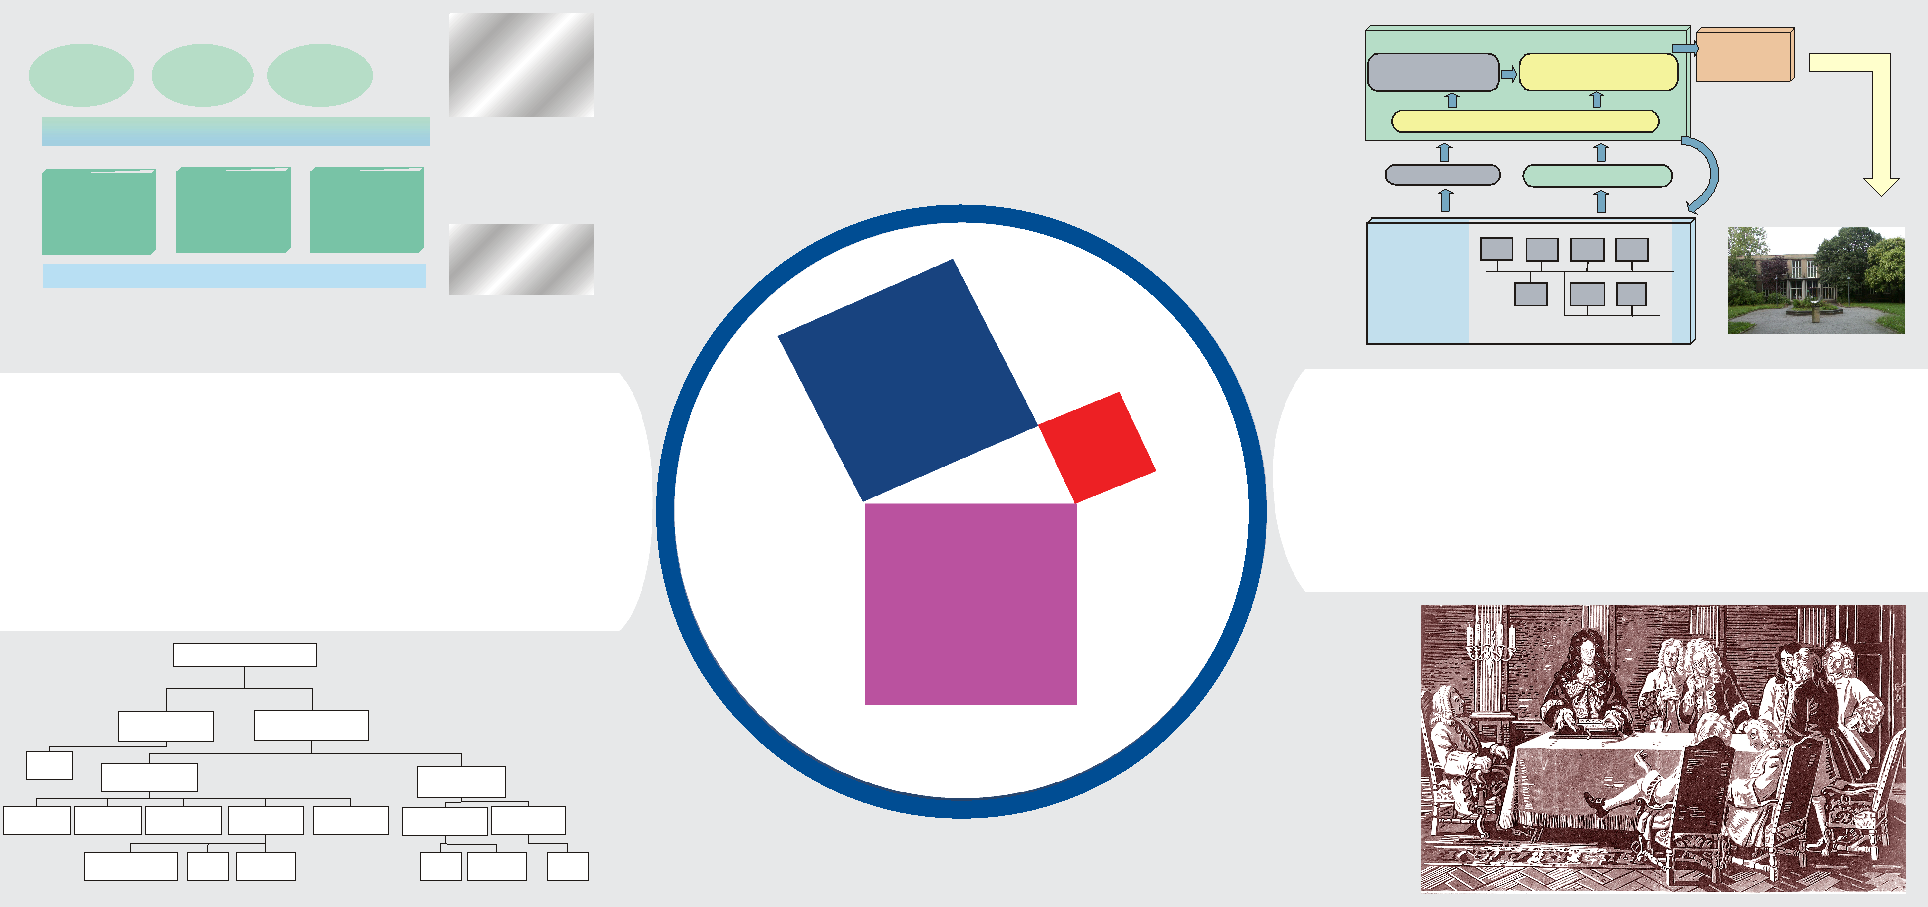
\includegraphics[width=\linewidth]{image2.png}
\centersection{Ausblick}

\begin{multicols}{2}
Auch Matrizen können unterschiedlich gefärbte Zeilen bekommen (müssen
aber nicht):\\\strut
\end{multicols}
\[
p^2=+\begin{pmatrix} a_1 &a_2\\a_3&a_4\end{pmatrix} = 
\begin{farbtabellen}\begin{pmatrix} a_1 &a_2\\a_3&a_4\end{pmatrix}\end{farbtabellen}
\]
\begin{multicols}{2}
  Lorem ipsum dolor sit amet, consectetuer adipiscing elit, sed diam nonummy nibh euismod tincidunt ut laoreet dolore Lorem ipsum dolor sit amet, consectetuer adipiscing elit, sed diam nonummy nibh euismod tincidunt ut laoreet dolore magna aliquam Lorem ipsum dolor sit amet, consectetuer adipiscing elit, sed diam nonummy nibh euismod tincidunt ut 
\end{multicols}
\pagebreak
\telefon{}%
\homepage{\strut http://www.math.tu-dresden.de/\textasciitilde schlemme/tudmathposter/}%
\email{\\ \strut Tobias.Schlemmer@mailbox.tu-dresden.de\\\strut}%
\title{2. Plakat}%
\subtitle{testausgaben}%
\maketitle
\section*{Test Aufzählung}
\begin{multicols}{2}
Dies ist eine Aufzählung.

\begin{itemize}
\item Item
\item Item
  \begin{itemize}
  \item SubItem
  \item SubItem
    \begin{itemize}
    \item SubSubItem
    \item SubSubItem
      \begin{itemize}
      \item SubSubSubItem
      \item SubSubSubItem
      \item SubSubSubItem
      \end{itemize}
    \item SubSubItem
    \end{itemize}
  \item SubItem
  \end{itemize}
\renewcommand*\labelitemi{\textbullet}
\item Item \vrule\kern1cm\vrule
\renewcommand*\labelitemi{\textbullet\,}
\item Item \vrule\kern1cm\vrule
\renewcommand*\labelitemi{\textbullet\kern 0.25em}
\item Item \vrule\kern1cm\vrule
\renewcommand*\labelitemi{\textbullet\,\,}
\item Item \vrule\kern1cm\vrule
\renewcommand*\labelitemi{\textbullet\enspace}
\item Item \vrule\kern1cm\vrule
\renewcommand*\labelitemi{\textbullet\kern 1em}
\item Item \vrule\kern1cm\vrule
\item[\raisebox{.2ex}{$\Rightarrow$}] Ergebnis
\end{itemize}

\section*{Test Buchstaben / Zahlen}
A B C D E F G H I J K L M N O P Q R S T U V W X Y Z Ä Ö Ü.
a b c d e f g h i j k l m n o p q r s t u v w x y z ä ö ü ß.
0 1 2 3 4 5 6 7 8 9.

\section*{Test Unterabschnitte}
\subsection*{Unterabschnitt 1}
Dies ist ein Absatz.
\subsection*{Unterabschnitt 2}
Dies ist ein noch ein Absatz.

\vfill
%\columnbreak
\section*{Test Mathematisches}
Vergleich Schriftart in Text und Formel:\\
1+2=3 vs. $1+2=3$.

Abgesetze Formeln:
\begin{eqnarray}
\mbox{Gleichung:}&&1+2*3-4/5\approx6\\
\mbox{Funktion:}&&A(r)=\pi r^2\\
\mbox{Funktionsnamen:}&&\lim_{n\to0}\frac{1}{n}=\infty\\
\mbox{Summensymbol:}&&e=\sum_{k=0}^{\infty}\frac{1}{k!}\\
\text{w$e$iter:}&&\int\limits_0^\pi \sin x\,dx = 2
\end{eqnarray}
a$a$a b$b$b c$c$c d$d$d e$e$e f$f$f g$g$g h$h$h i$i$i j$j$j k$k$k
l$l$l m$m$m n$n$n o$o$o p$p$p q$q$q r$r$r s$s$s t$t$t u$u$u v$v$v
w$w$w x$x$x y$y$y z$z$z 1$1$1 2$2$2 3$3$3 4$4$4 5$5$5 6$6$6 7$7$7
8$8$8 9$9$9 0$0$0 A$A$A B$B$B C$C$C E$E$E F$F$F G$G$G H$H$H I$I$I
J$J$J K$K$K L$L$L M$M$M N$N$N O$O$O P$P$P Q$Q$Q R$R$R S$S$S T$T$T
U$U$U V$V$V W$W$W X$X$X Y$Y$Y Z$Z$Z $R\mathbb RR$ $\partial x$
$G\Gamma D\Delta T\Theta L\Lambda X\Xi P\Pi S\Sigma Y\Upsilon F\Phi
Ps\Psi O\Omega s\sigma r\rho$ 
\[
\mathbf{\frac{\text{A}ABCDEFGHI\mathfrak{JKLM}NOPQRSTUVWXYZ\text{Z}}
{\text{a}abcdefghijklmnopqrstuvwxyz\text{z}}}
\]
$!$!$($($)$)$+$+$-$-$=$=$[$[$]$]$"$"$\&$\&$:$:$;$;$?$?$`$`$|$|
$\aleph\Re\Im\neg=\neq\wedge\vee\setminus\sim\mid\mathsection$
$\intop\ointop\braceld\bracerd\bracelu\braceru\infty\nearrow\searrow\nwarrow\swarrow$
$\Leftrightarrow\Leftarrow\Rightarrow\leftrightarrow\rightarrow\leftharpoonup\leftharpoondown$

\vfill
%\columnbreak
\section*{Test Grafik}
\rule{\linewidth}{2cm}
\end{multicols}


\iffalse
%\definecolor{mathelogoblau}{cmyk}{0.96,0.7,0.00,0.07}
%\definecolor{mathelogorot}{cmyk}{0.00,0.99,0.95,0.00}
%\definecolor{mathelogoviolett}{cmyk}{0.27,0.99,0.00,0.03}
% das sollte man nicht machen, da für den Druck cmyk gebraucht wird
% aber ich habe nur RGB
\definecolor{mathelogoblau}{rgb}{0.0392,0.2784,0.9294}
\definecolor{mathelogorot}{rgb}{1,0.0117,0.051}
\definecolor{mathelogoviolett}{rgb}{0.7098,0.0117,0.9686}

\begin{tikzpicture}[scale=4]
\fill [mathelogoviolett] (0,0) rectangle (1,-1);
\fill [mathelogoblau,rotate=36.8] (0,0) rectangle (0.8,0.8);
\fill [mathelogorot,rotate around={-53:(1,0)}] (0.4,0) rectangle (1,0.6);
\end{tikzpicture}
\fi
\Huge Huge $2^{2^2}$

\huge huge $2^{2^2}$

\LARGE LARGE  $2^{2^2}$

\Large Large $2^{2^2}$

\large large $2^{2^2}$

\normalsize normalsize $2^{2^2}$

\small small $2^{2^2}$

\footnotesize footnotesize $2^{2^2}$

\scriptsize scriptsize $2^{2^2}$

\tiny tiny $2^{2^2}$

\vfill
Diese Hilfslinie zeigt das Seitenende an. \textbf{ZU ENTFERNEN}!
\hrule

\end{document}
